\subsection{استخراج قسمت های کوچیک تر از یک اسلاید}\label{subsec:استخراج-قسمت-های-کوچیک-تر-از-یک-اسلاید}

اسلاید هایی که متخصصان از آن برای تشخیص استفاده می کنند بسیار ابعاد بزرگی دارند، به طوری که به هیچ وجه در
حافظه پردازنده ها جای نمی گیرد.
برای حل این مشکل در این پروژه سعی بر این شد که اسلاید‌ها به تیکه‌های کوچک تری از عکس شکسته شوند به طوری که قابل پردازش باشند.
یکی از موضوعات مهمی که باید در نظر گرفت، ناحیه‌های غیر مهم و فاقد اطلاعات است که باید در این فرآیند حذف گردند. این کار به دو دلیل انجام می شود.
اولا اینکه این قسمت‌ها، بخش بزرگی از اسلاید‌ها را تشکیل می دهند و با حذف این موارد می توان در استفاده از منابع پردازشی صرفه جویی کرد
و دوما اگر تعداد زیادی از عکس‌هایی که هنگام آموزش مدل استفاده می کنیم، از این نوع باشند، دقت مدل بشدت کاهش پیدا می کند و مدل در فرآیند یادگیری با مشکل مواجه می شود.
دلیل این امر هم این است که این عکس‌ها حاوی ویژگی‌های مورد نظر ما برای تشخیص سلول‌های سرطانی نیستند و مدل در حین فرآیند آموزش، ویژگی‌های نامربوطی را از روی این عکس‌ها یاد می گیرد.

برای حل این موضوع، روشی که بکار گرفته شد، استفاده از واریانیس لاپلاسین ناحیه است.
لاپلاسین یک عکس از محاسبه مشتق دوم روی شدت رنگ‌های پیکسل‌های آن محاسبه می شود
و در نتیجه لبه و گوشه‌های عکس مقدار بیشتری می گیرد.
برای محاسبه مشتق دوم برای یک عکس از رابطه زیر استفاده می کنیم که در آن $f(x)$ مقدار شدت رنگ را در موقعیت x از تصویر نشان می دهد.

\begin{gather*}
    f'(x) = f(x+1) - f(x), f'(x+1) = f(x+2) - f(x+1)\\
    f"(x) = f'(x+1) - f'(x)= f(x+2) - f(x+1) - f(x+1) + f(x)\\
    f"(x) = f(x+2) - 2*f(x+1) + f(x)\\
\end{gather*}

بعد از محاسبه واریانس شدت رنگ پیکسل‌ها در لاپلاسین عکس و استفاده از یک آستانه عکس‌هایی که مقدار کمتری دارند فیلتر می شوند.
به این ترتیب ناحیه‌های فاقد اطلاعات که مقدار لاپلاسین کمی نیز دارند حذف می شوند.

برای بدست آوردن مقدار بهینه آستانه و همچنین آزمودن این روش، به ترتیب زیر عمل شد.
\begin{enumerate}
    \item ابتدا حدس اولیه 500 برای آستانه انتخاب شد و اسلاید‌ها با توجه به این آستانه به قطعه‌های کوچک عکس در آمدند.
    مقدا اولیه آستانه در این مرحله، نیاز به دقت بالایی ندارد، زیرا همانطور که در قسمت بعد نیز توضیح داده خواهد شد، از آن برای انتخاب اسلاید‌ها استفاده می کنیم.
    این حدس اولیه نیز با مشاهده مقدار به صورت حدودی و از روی چند ناحیه تصادفی از یک اسلاید انتخاب شد.
    توزیع تعداد و درصد قطعه عکس‌های هر اسلاید در تصویر~\رجوع{شکل: توزیع تعداد و درصد قطعه عکس‌های هر اسلاید با آستانه 500} آمده است.
    \begin{figure}
        \begin{center}
            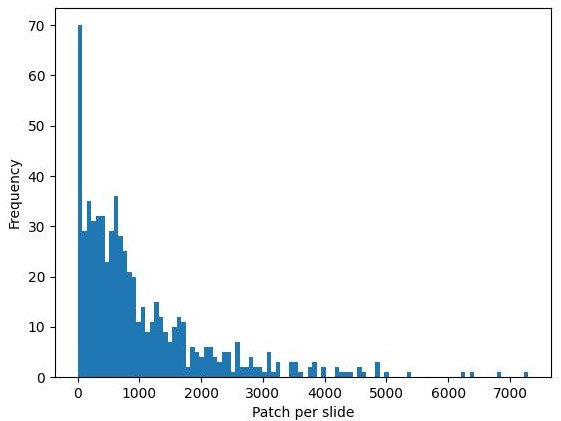
\includegraphics[width=0.48\linewidth]{figs/introduction/subs/challenges/patch_distribution_old_500_threshold.jpeg}
            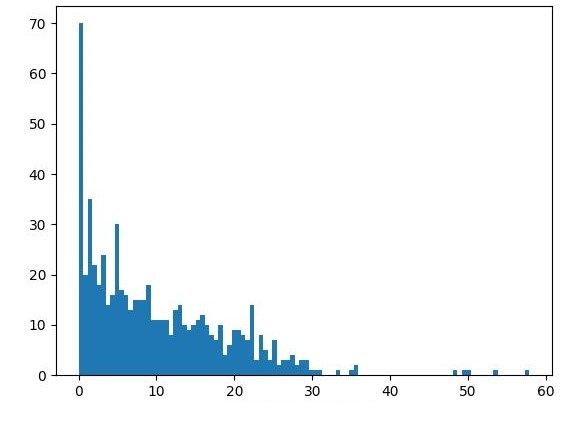
\includegraphics[width=0.48\linewidth]{figs/introduction/subs/challenges/patch_percent_distribution_old_threshold_500.jpeg}
            \hspace{.2cm}
            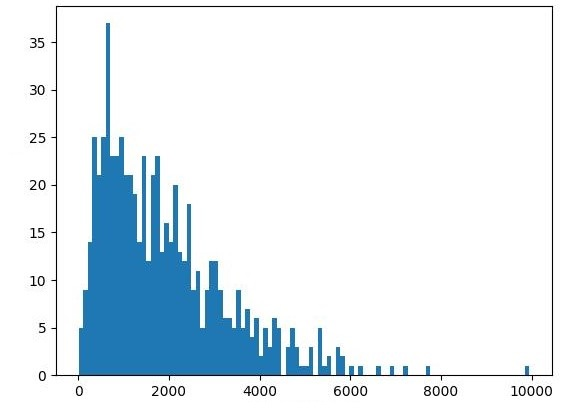
\includegraphics[width=0.48\linewidth]{figs/introduction/subs/challenges/patch_distribution_new_298_threshold.jpeg}
            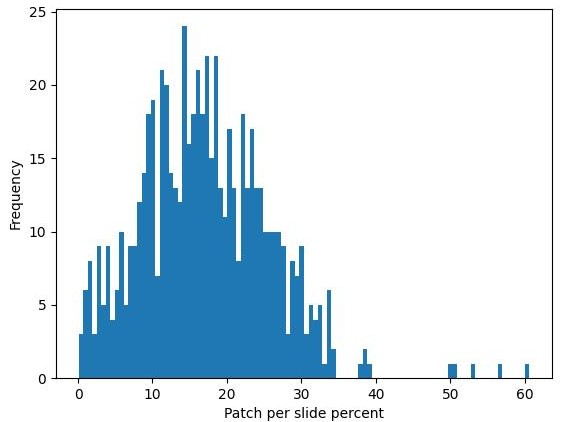
\includegraphics[width=0.48\linewidth]{figs/introduction/subs/challenges/patch_percent_distribution_new_threshold_298.jpeg}
        \end{center}
        \caption{نمودار‌ها به ترتیب از راست به چپ توزیع تعداد قطعه عکس‌های تولید شده از هر اسلاید و درصد قطعه عکس‌های تولید شده نسبت به تعداد کل را برای هر اسلاید با آستانه 500 و 298 نشان می دهد.}
        \label{شکل: توزیع تعداد و درصد قطعه عکس‌های هر اسلاید با آستانه 500}
    \end{figure}
    \item سپس سه اسلاید از پایین بازه و سه اسلاید از بالای بازه مشخص شده در نمودار توزیع قطعه عکس‌ها انتخاب شدند.
    سه اسلاید بالای بازه اسلاید‌هایی هستند که روش بکار رفته تعداد زیادی قطعه عکس از آن‌ها تولید کرده است و سه اسلاید پایین بازه اسلاید‌هایی هستند که به دلیل نابهینه بودن آستانه، روش ما، قطعه عکس‌های کمی را برای آن‌ها تولید کرده است.
    \item برای شش اسلاید انتخاب شده، به صورت دستی و با استفاده از نرم افزار GIMP ماسک‌هایی تولید شد.
    \item در قدم بعد، باید معیار‌هایی را برای روش بکار رفته انتخاب کرد تا با استفاده از آن‌ها بتوان آستانه بهینه را پیدا کرد و در نهایت آن را ارزیابی کرد.
    همانطور که در قسمت‌های قبل گفته شد، فیلتر ناحیه‌های فاقد اطلاعات، اهمیت زیادی برای ما دارد از این رو، در ارزیابی این روش علاوه بر دقت\LTRfootnote{Accuracy}، صحت\LTRfootnote{Precision} نیز عامل مهمی در کارکرد درست است.
    صحت، با توجه به فرمول زیر هرچه به مقدار عددی 1 نزدیک تر باشد به این معناست که ناحیه‌های بدست آمده از این روش، به احتمال بالاتری دارای اطلاعات هستند و در نتیجه ناحیه‌های فاقد اطلاعات کمتری تولید می شوند.
    \begin{gather*}
        TruePositive(TP) :\textit{روش به درستی عکس را غیر پس زمینه تشخیص داده}\\
        TrueNegative(TN) :\textit{ روش به درستی عکس را پس زمینه تشخیص داده}\\
        FalsePositive(FP) :\textit{ روش اشتباهاً عکس را غیر پس زمینه تشخیص داده}\\
        FalseNegative(FN) :\textit{ روش اشتباهاً عکس را پس زمینه تشخیص داده}\\
        Precision = \frac{TP}{TP + FP}\\
    \end{gather*}
    دقت روش نیز به صورت زیر محاسبه می شود:
    \[Accuracy = \frac{TP + TN}{TP + FP + TN + FN}\]
    \item حال با توجه به این دو معیار، قطعه کد پایتونی نوشته شد که شش اسلاید و ماسک‌های مربوط به آن‌ها را به عنوان ورودی می گیرد و با شروع از آستانه 500 و محاسبه ماتریس درهم ریختگی\LTRfootnote{Confusion Matrix}، در جهتی آستانه را تغییر می دهد تا دو معیار گفته شده بیشینه شوند.
    لازم به ذکر است، در نهایت از تابع هدف\LTRfootnote{Objective Function} $0.25*Precision+0.75*Accuracy$ برای یافتن آستانه استفاده شد تا صحت مقدار پایینی به خود نگیرد.
    در هر مرحله از اجرای کد، از هر اسلاید 2000 و در مجموع $2000 * 6$ قطعه عکس مورد بررسی قرار می گیرد به صورتی که آستانه در جهت افزایش تابع هدف و با اندازه پرش\LTRfootnote{Jump Size} $120$ و نرخ نزولی\LTRfootnote{Decay Rate} $0.85$، کاهش و یا افزایش پیدا می کند.
    نمودار تغییرات تابع هدف و آستانه در طی اجرای برنامه در تصویر~\رجوع{شکل: تغیرات تابع هدف و آستانه در طول اجرا} آمده است که در آن‌ها تابع هدف و آستانه به ترتیب به مقادیر $0.96$ و $298$ همگرا شده اند.
    \begin{figure}
        \begin{center}
            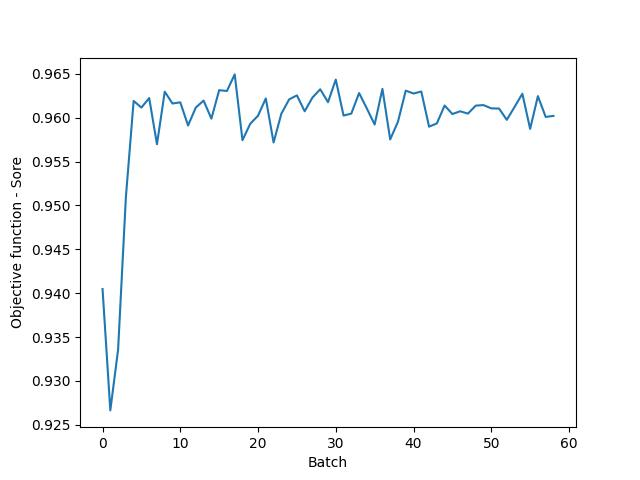
\includegraphics[width=0.48\linewidth]{figs/introduction/subs/challenges/laplacian_threshold_score_history_chart.jpeg}
            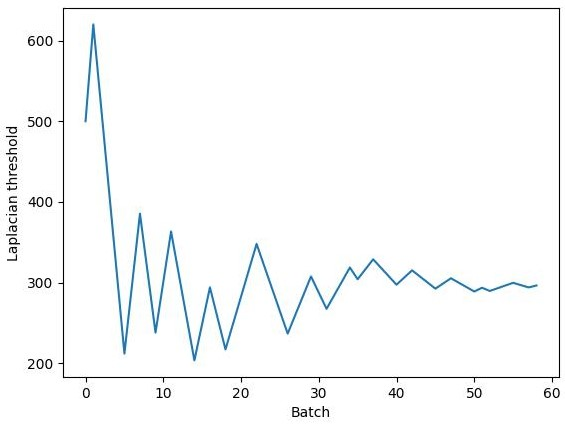
\includegraphics[width=0.48\linewidth]{figs/introduction/subs/challenges/laplacian_threshold_history_chart.jpeg}
        \end{center}
        \caption{به ترتیب از راست به چپ، تغیرات تابع هدف و آستانه قابل مشاهده است که در نهایت آستانه به مقدار 298 همگرا شده است.}
        \label{شکل: تغیرات تابع هدف و آستانه در طول اجرا}
    \end{figure}
    اسلاید‌ها و ماسک‌های بکار رفته آن‌ها در تصویر~\رجوع{شکل: شش اسلاید و ماسک‌های مرتبط} ارائه شده است و دقت و حساسیت روش بر روی این شش اسلاید نیز در جدول~\رجوع{جدول: دقت روش لاپلاسین بر روی شش اسلاید} آمده است.
    \begin{table}[t]
        \centering
        \begin{latin}
            \begin{tabular}{|c|l|c|c|c|}
                \hline
                \rl{اسلاید} & \rl{{ماتریس درهم ریختگی}} & \rl{دقت} & \rl{صحت}
                \\
                \hline
                \hline
                \textit{1} & \textit{TP: $4624$  FP: $126$ TN: $14100$ FN: $226$} & $0.98$ & $0.97$\\
                \textit{2} & \textit{TP: $1103$  FP: $172$ TN: $3758$  FN: $7$} & $0.96$ & $0.86$\\
                \textit{3} & \textit{TP: $7615$  FP: $92$  TN: $20871$ FN: $234$} & $0.98$ & $0.98$\\
                \textit{4} & \textit{TP: $78$    FP: $18$  TN: $1880$  FN: $4$} & $0.98$ & $0.81$\\
                \textit{5} & \textit{TP: $1138$  FP: $4$   TN: $6671$  FN: $492$} & $0.94$ & $0.99$\\
                \textit{6} & \textit{TP: $460$   FP: $0$   TN: $19618$ FN: $1426$} & $0.93$ & $0.99$\\
                \hline
                \textit{In Total} & \textit{TP: $15018$ FP: $412$ TN: $66898$ FN: $2389$} & $0.96$ & $0.97$\\
                \hline
            \end{tabular}
        \end{latin}
        \caption{دقت روش لاپلاسین برای تشخیص عکس‌های پس زمینه از غیر پس زمینه}
        \label{جدول: دقت روش لاپلاسین بر روی شش اسلاید}
    \end{table}

    \begin{figure}
        \begin{center}
            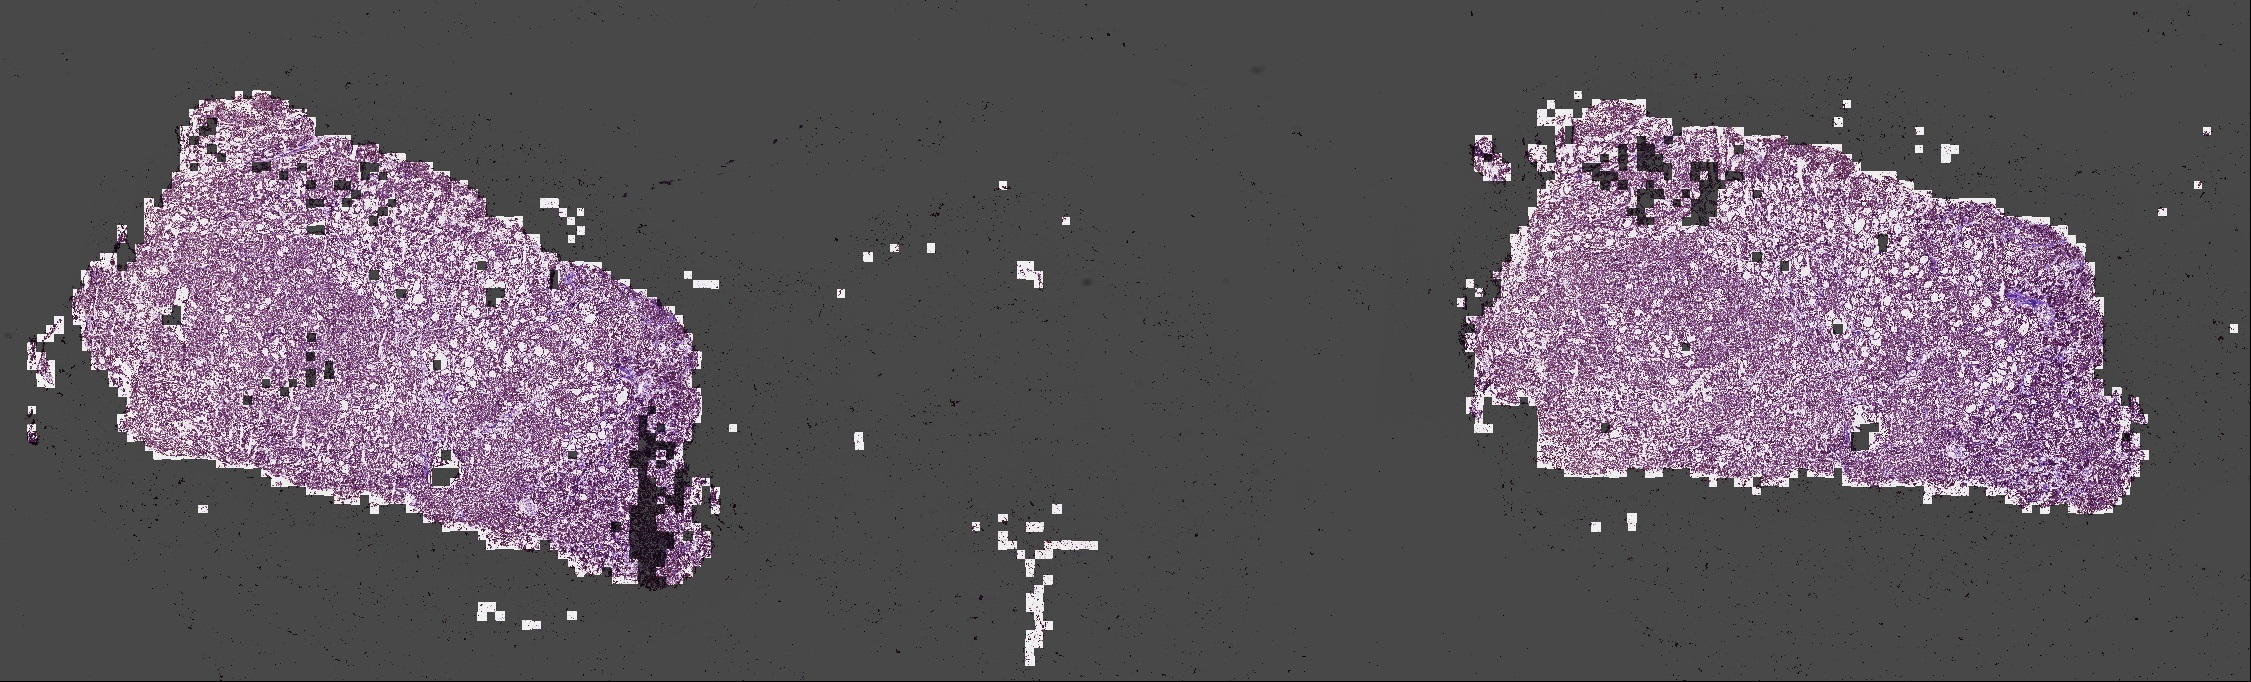
\includegraphics[width=0.48\linewidth]{figs/introduction/subs/challenges/evaluate_slides/TCGA-DJ-A1QG-01A-01-TSA.04c62c21-dd45-49ea-a74f-53822defe097__2000_generated_mask.jpg}
            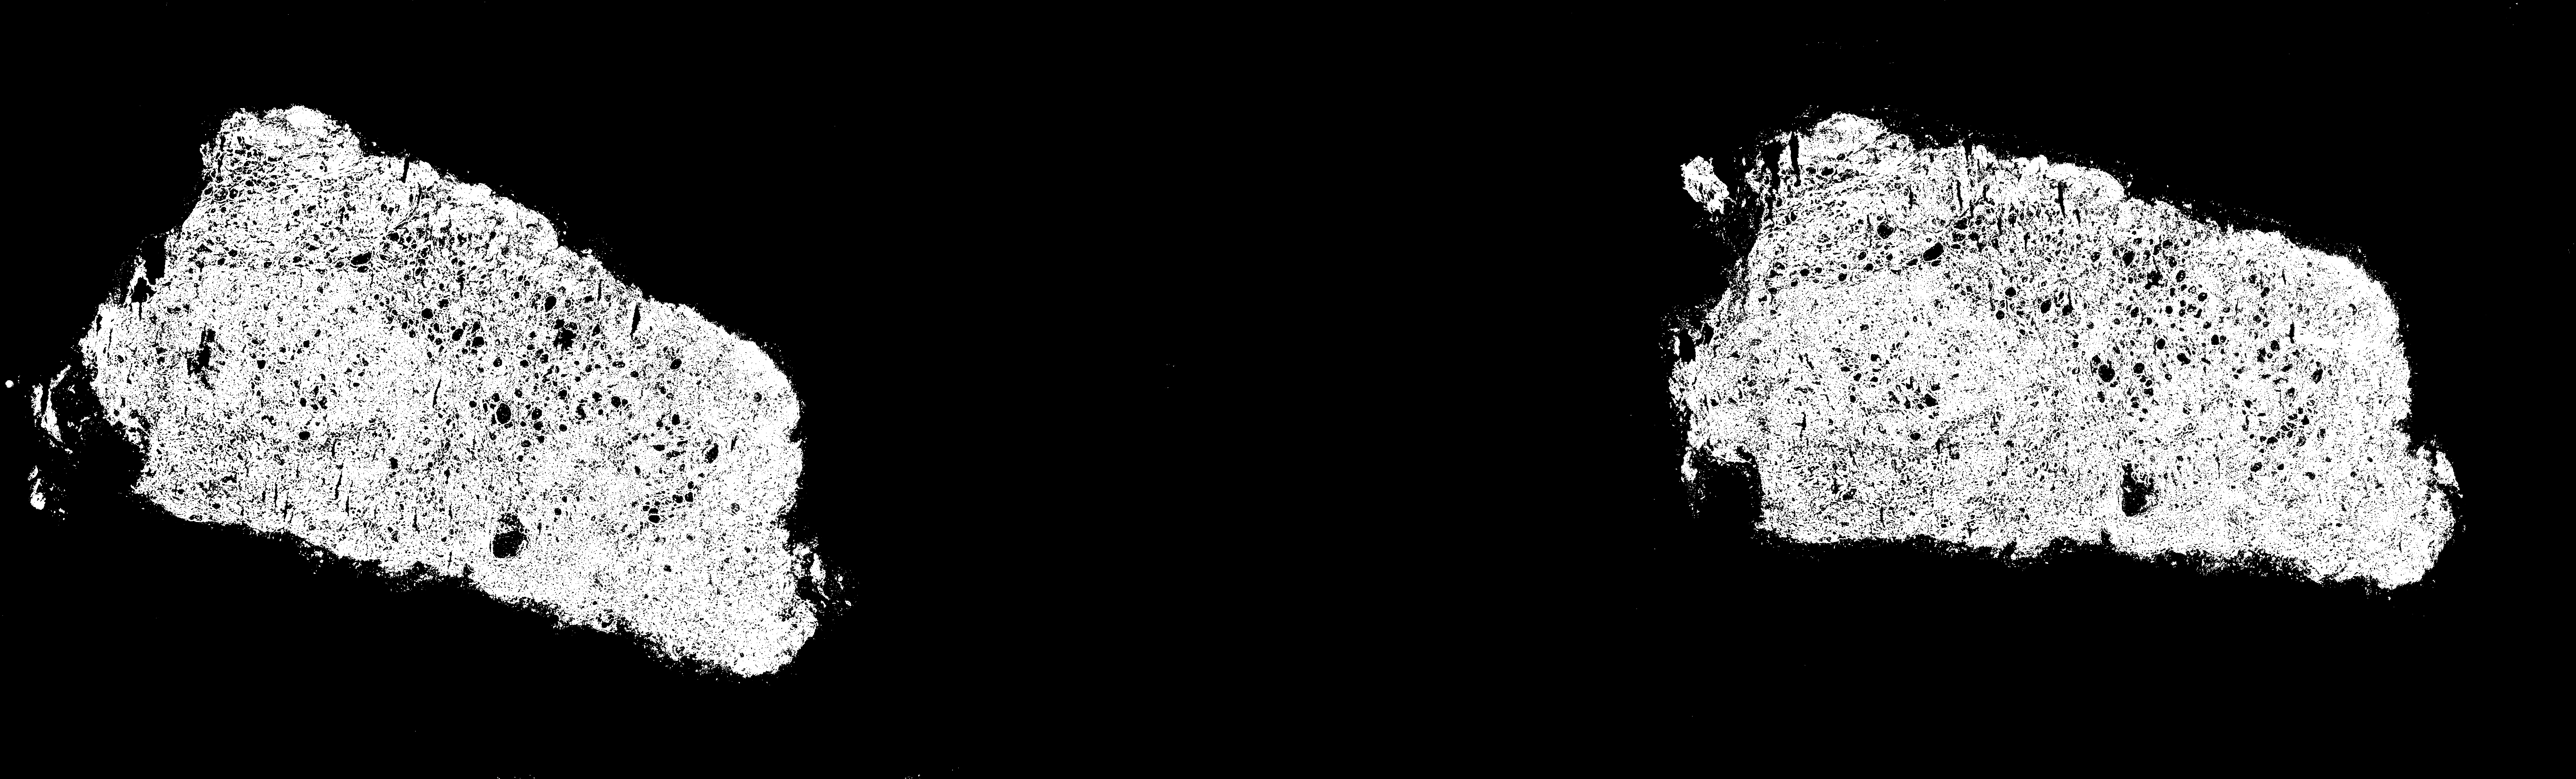
\includegraphics[width=0.48\linewidth]{figs/introduction/subs/challenges/evaluate_slides/TCGA-DJ-A1QG-01A-01-TSA.04c62c21-dd45-49ea-a74f-53822defe097__2000_masked.png}
            \hspace{.2cm}
            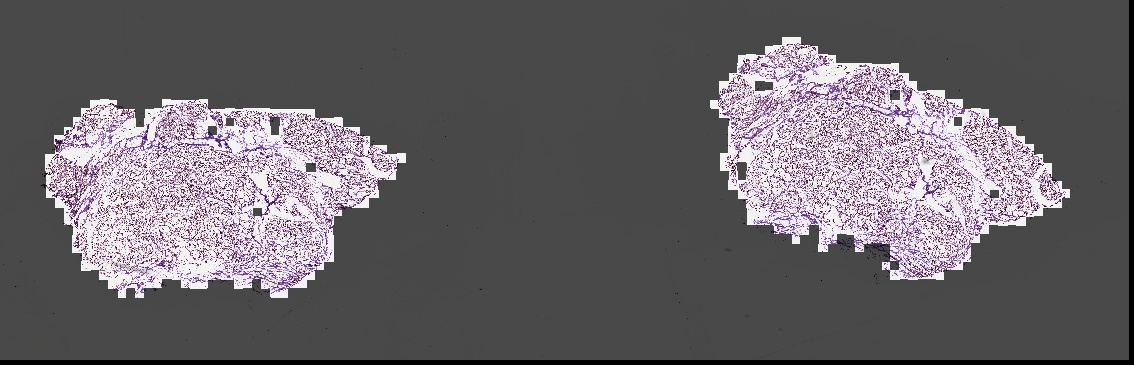
\includegraphics[width=0.48\linewidth]{figs/introduction/subs/challenges/evaluate_slides/TCGA-EL-A3TB-11A-01-TS1.6E0966C9-1552-4B30-9008-8ACF737CA8C3__2000_generated_mask.jpg}
            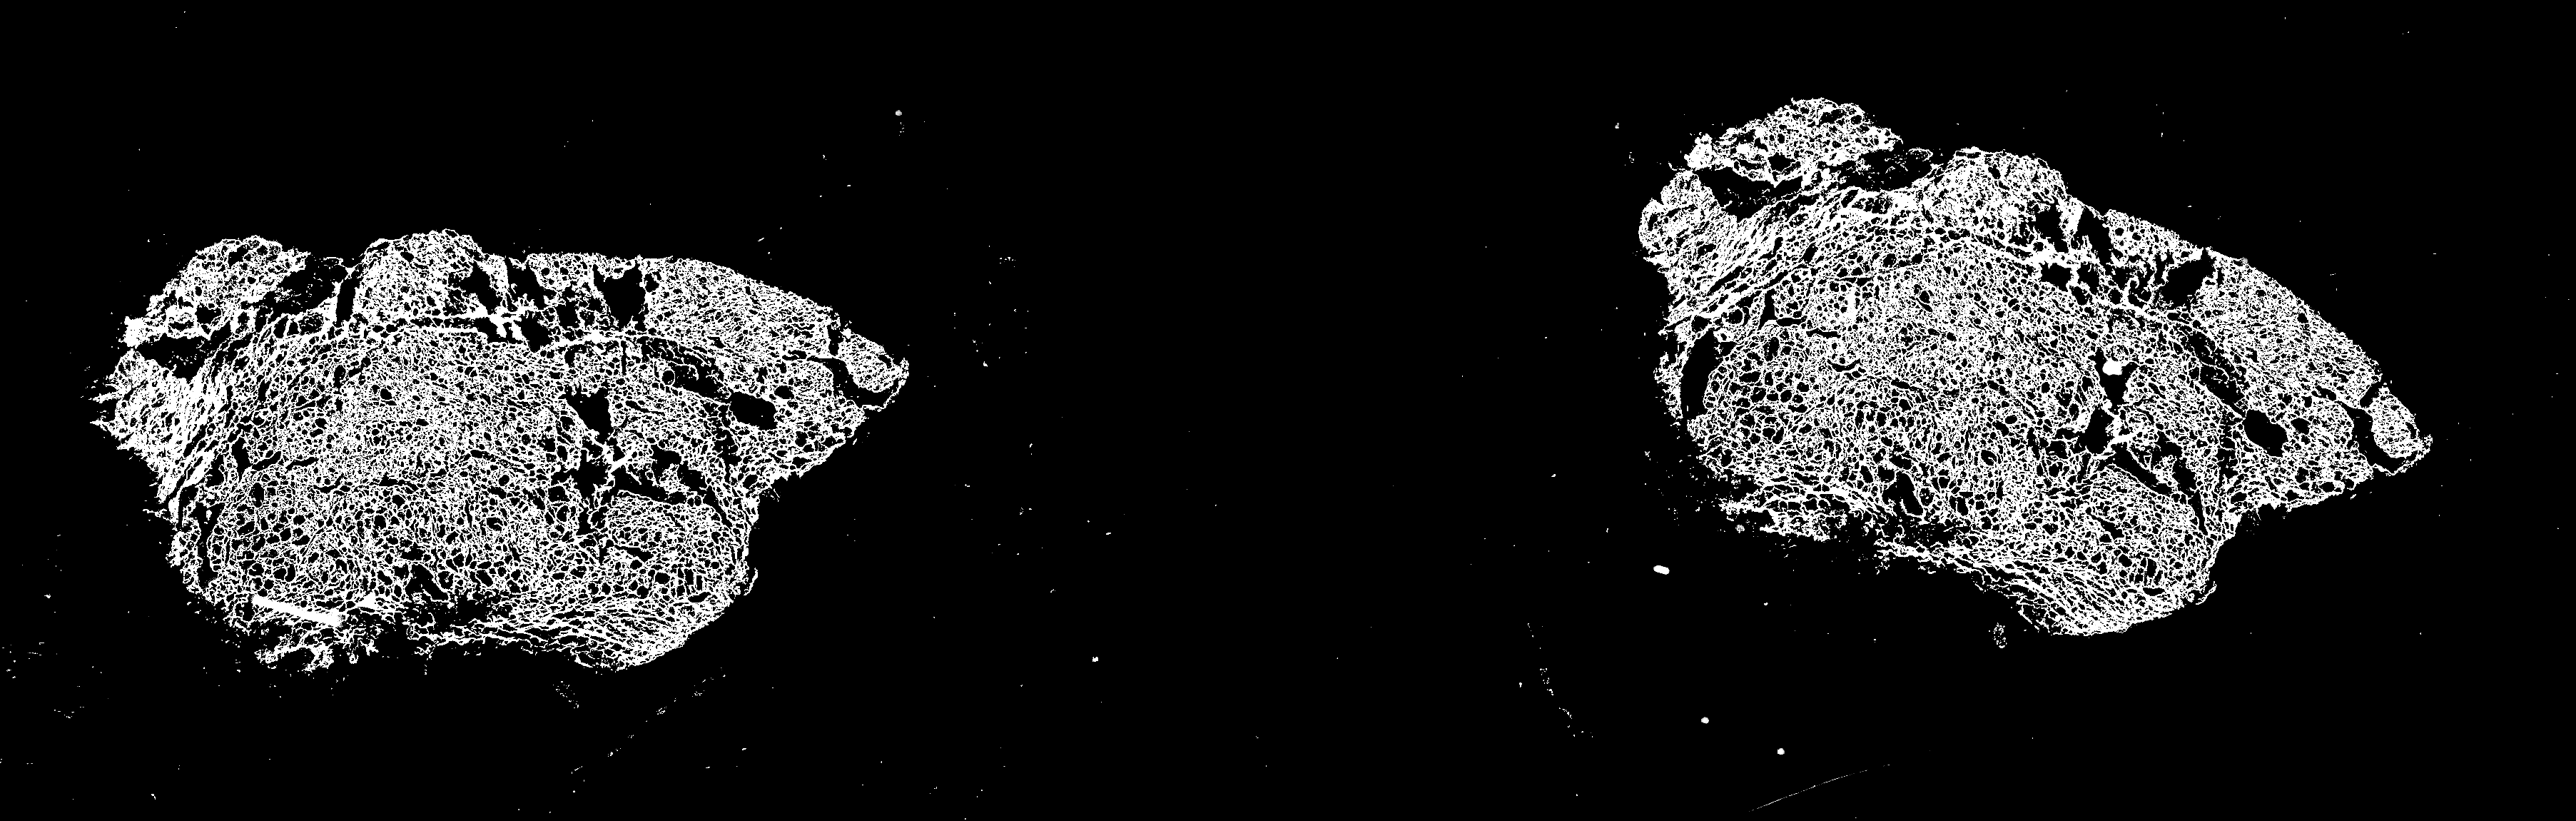
\includegraphics[width=0.48\linewidth]{figs/introduction/subs/challenges/evaluate_slides/TCGA-EL-A3TB-11A-01-TS1.6E0966C9-1552-4B30-9008-8ACF737CA8C3__2000_masked.png}
            \hspace{.2cm}
            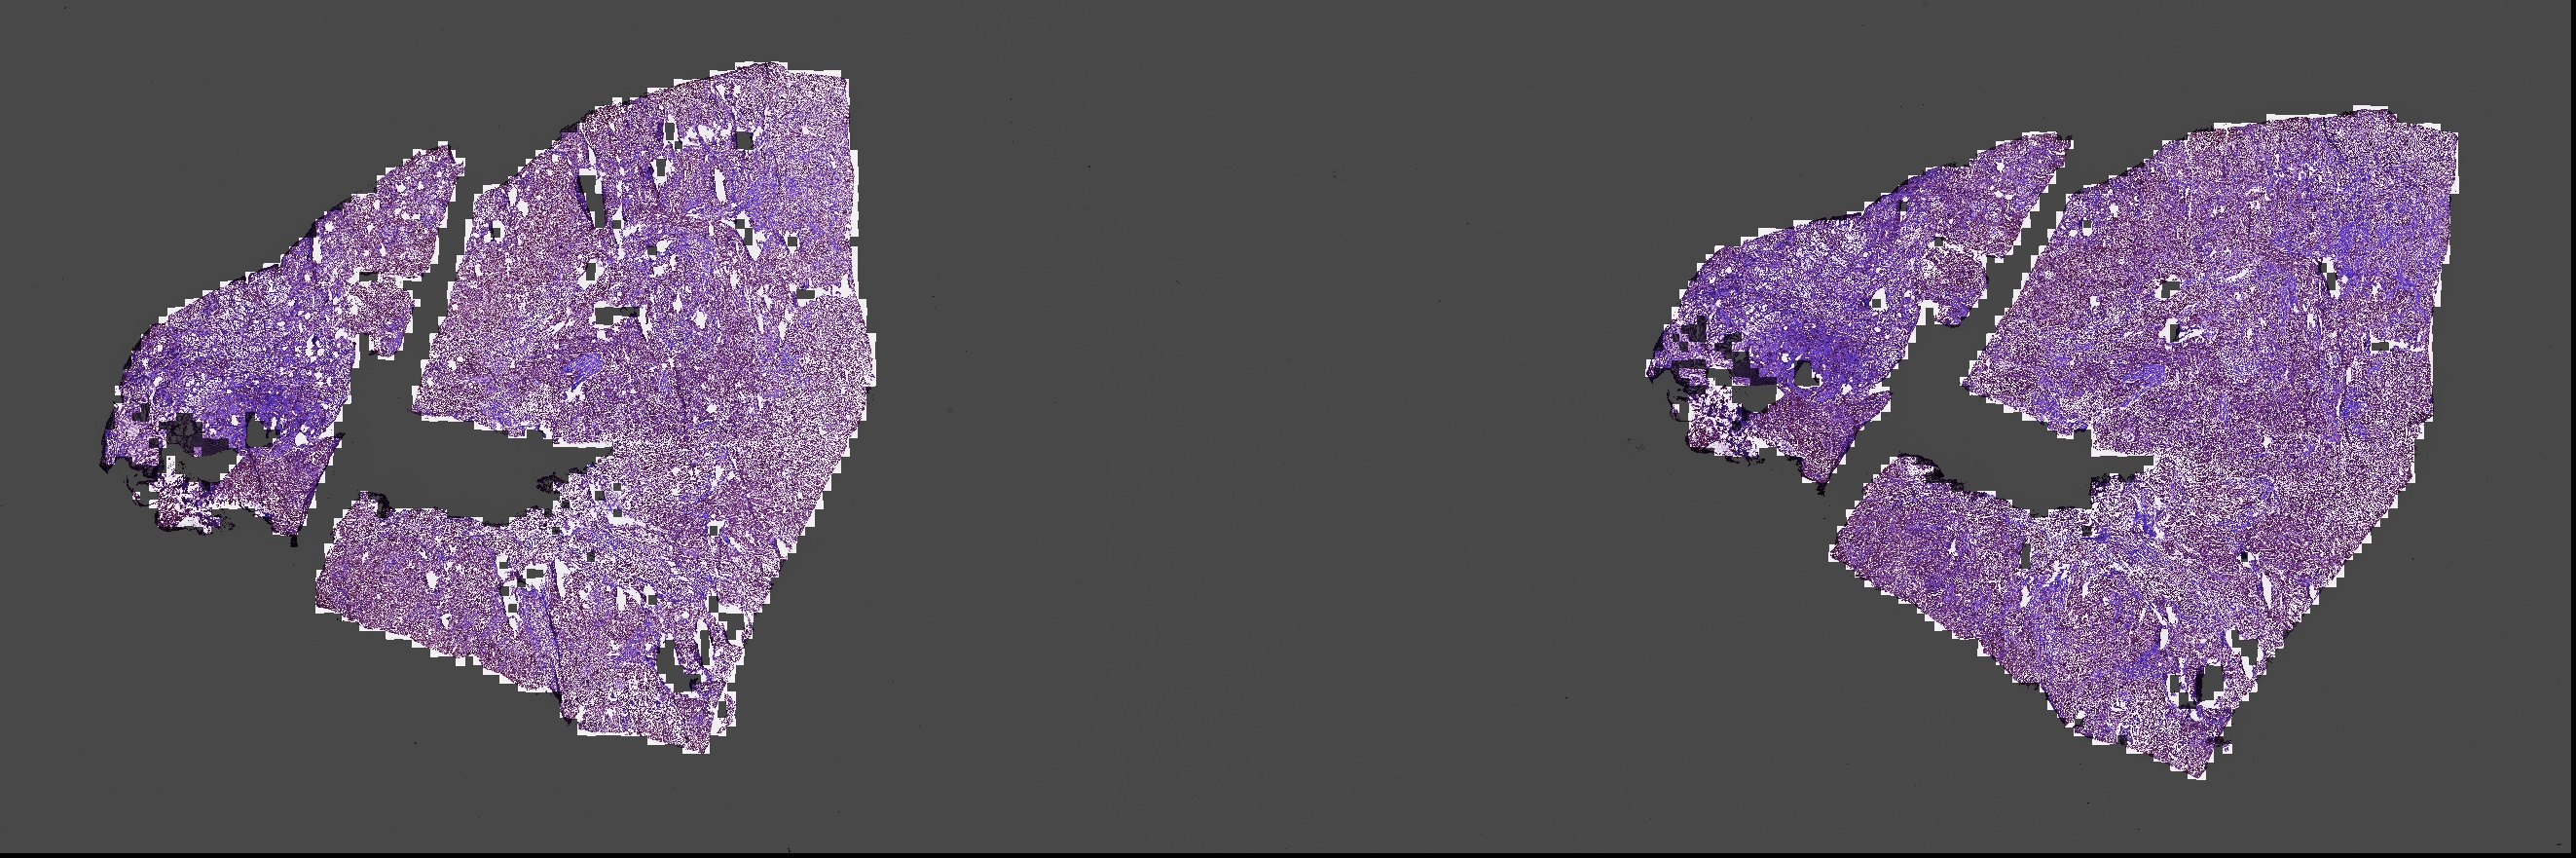
\includegraphics[width=0.48\linewidth]{figs/introduction/subs/challenges/evaluate_slides/TCGA-ET-A39O-01A-01-TSA.3829C900-7597-4EA9-AFC7-AA238221CE69_7000_generated_mask.jpg}
            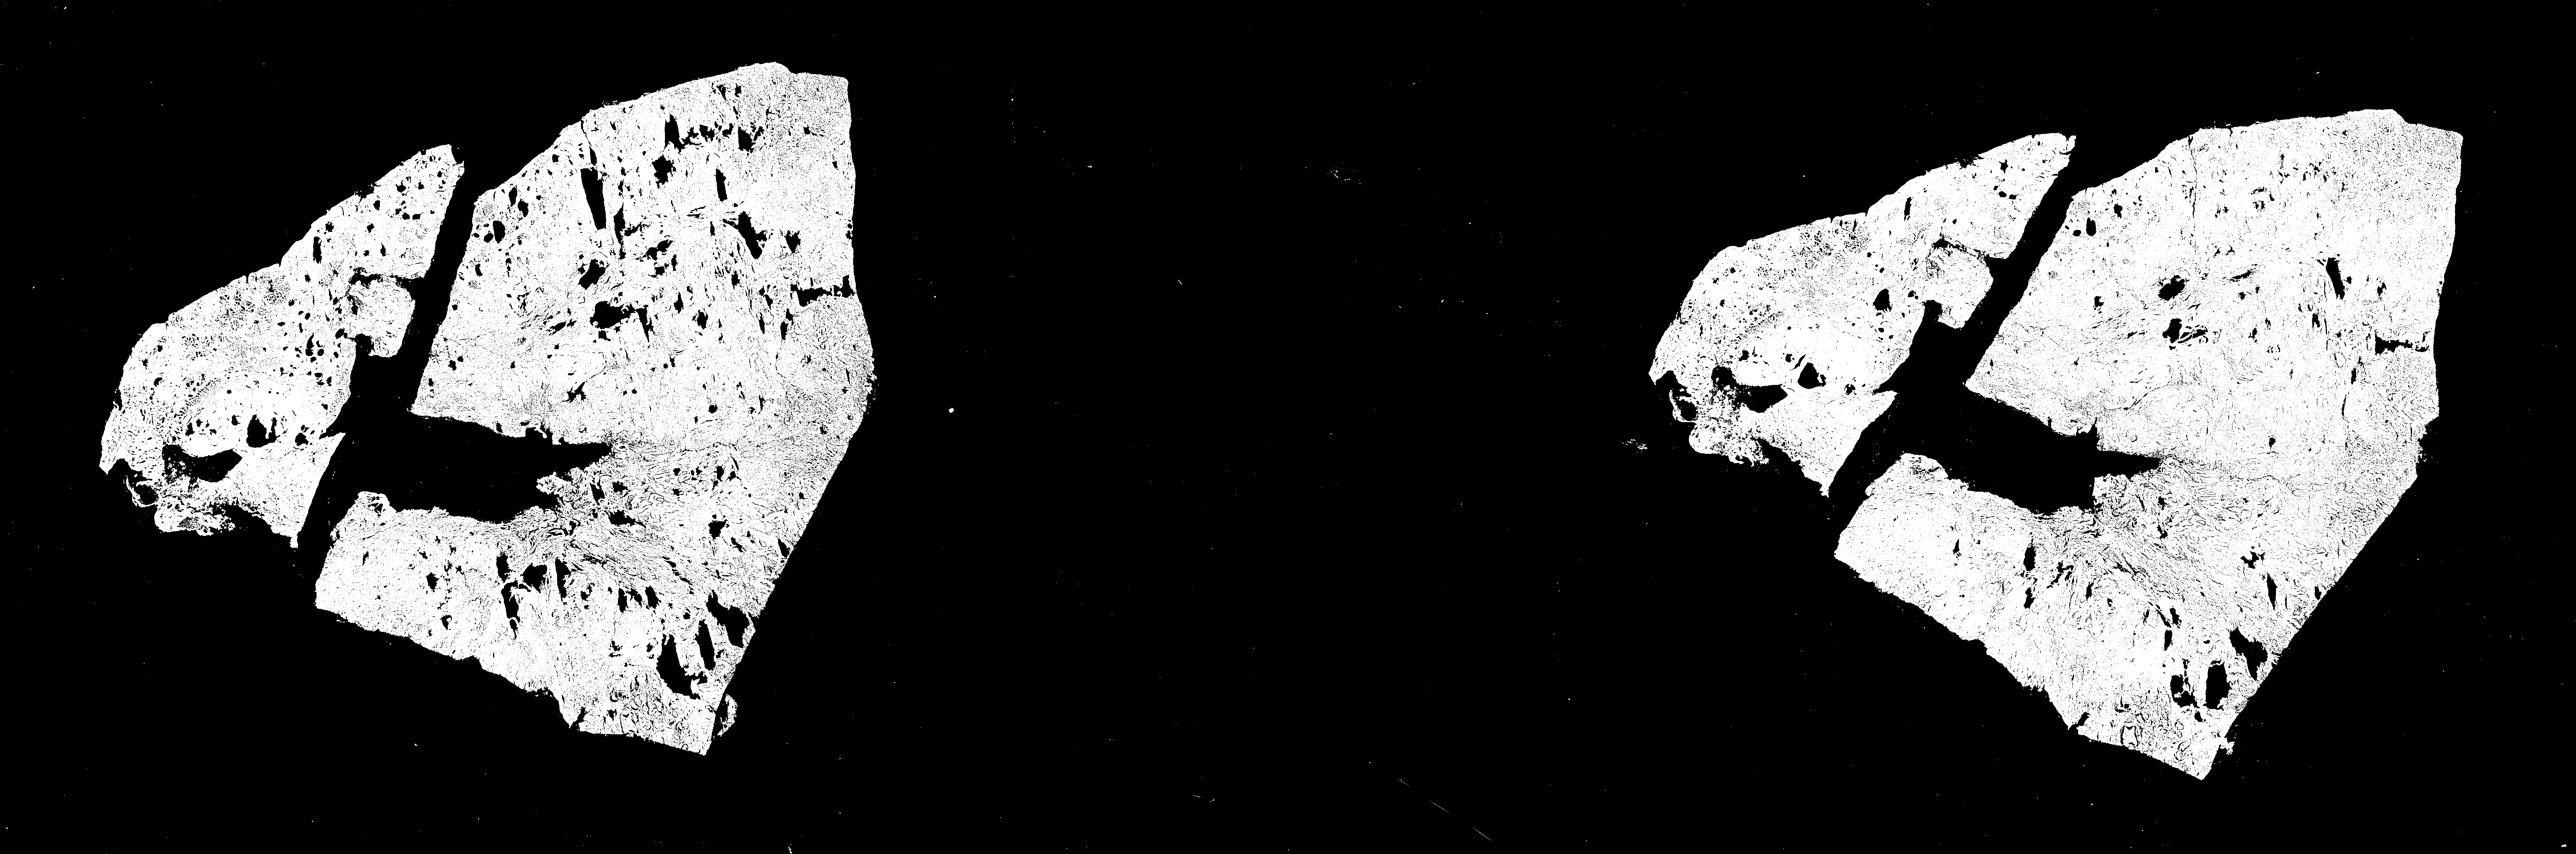
\includegraphics[width=0.48\linewidth]{figs/introduction/subs/challenges/evaluate_slides/TCGA-ET-A39O-01A-01-TSA.3829C900-7597-4EA9-AFC7-AA238221CE69_7000_masked.png}
            \hspace{.2cm}
            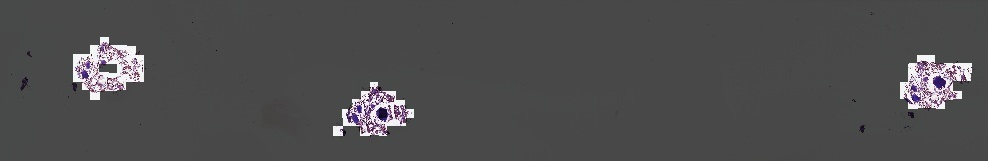
\includegraphics[width=0.48\linewidth]{figs/introduction/subs/challenges/evaluate_slides/TCGA-EL-A4K7-11A-01-TS1.C08B59AA-87DF-4ABB-8B70-25FEF9893C7F__70_generated_mask.jpg}
            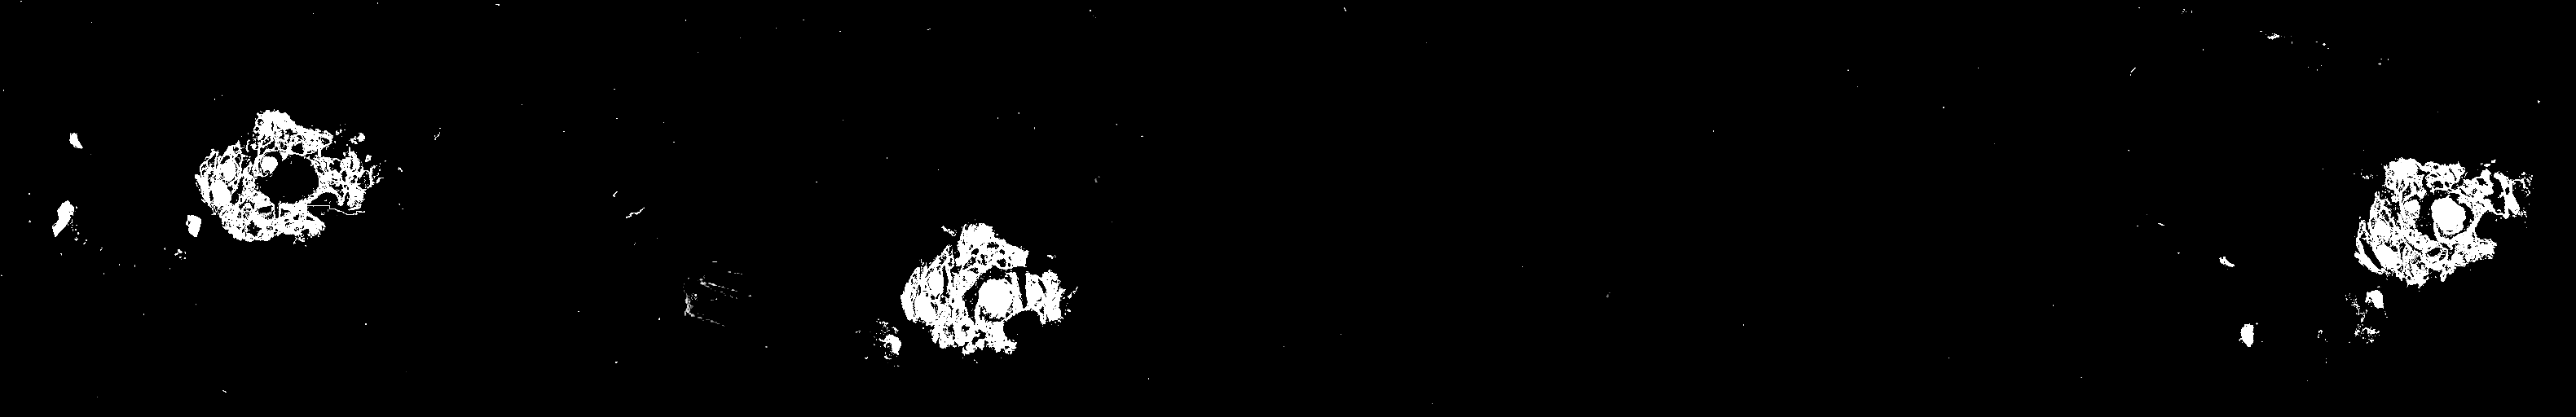
\includegraphics[width=0.48\linewidth]{figs/introduction/subs/challenges/evaluate_slides/TCGA-EL-A4K7-11A-01-TS1.C08B59AA-87DF-4ABB-8B70-25FEF9893C7F__70_masked.png}
            \hspace{.2cm}
            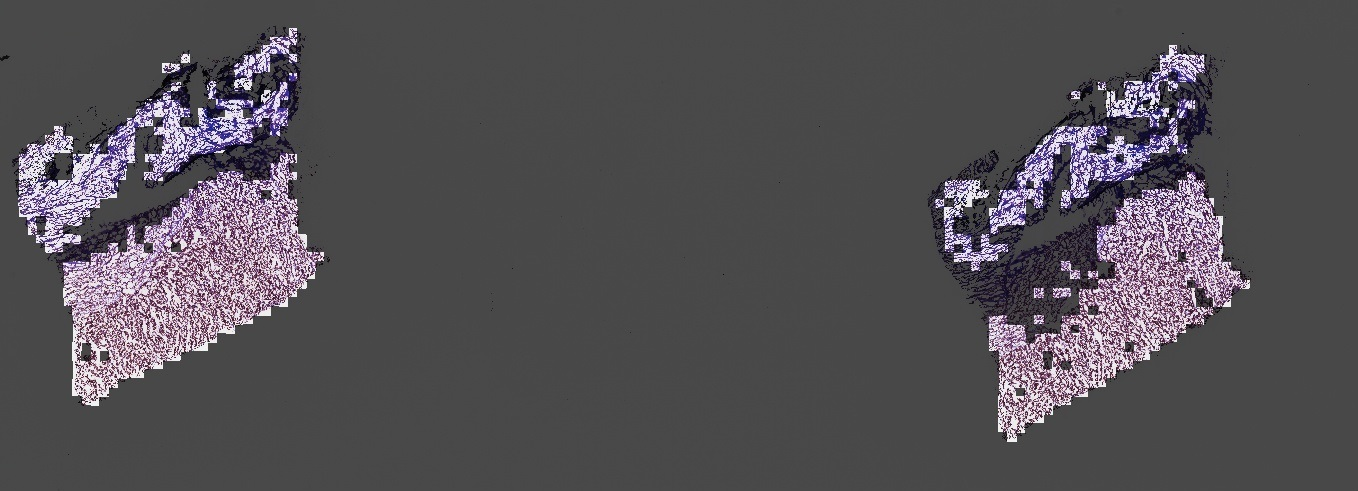
\includegraphics[width=0.48\linewidth]{figs/introduction/subs/challenges/evaluate_slides/TCGA-ET-A39N-01A-01-TSA.C38FCE19-9558-4035-9F0B-AD05B9BE321D___198_generated_mask.jpg}
            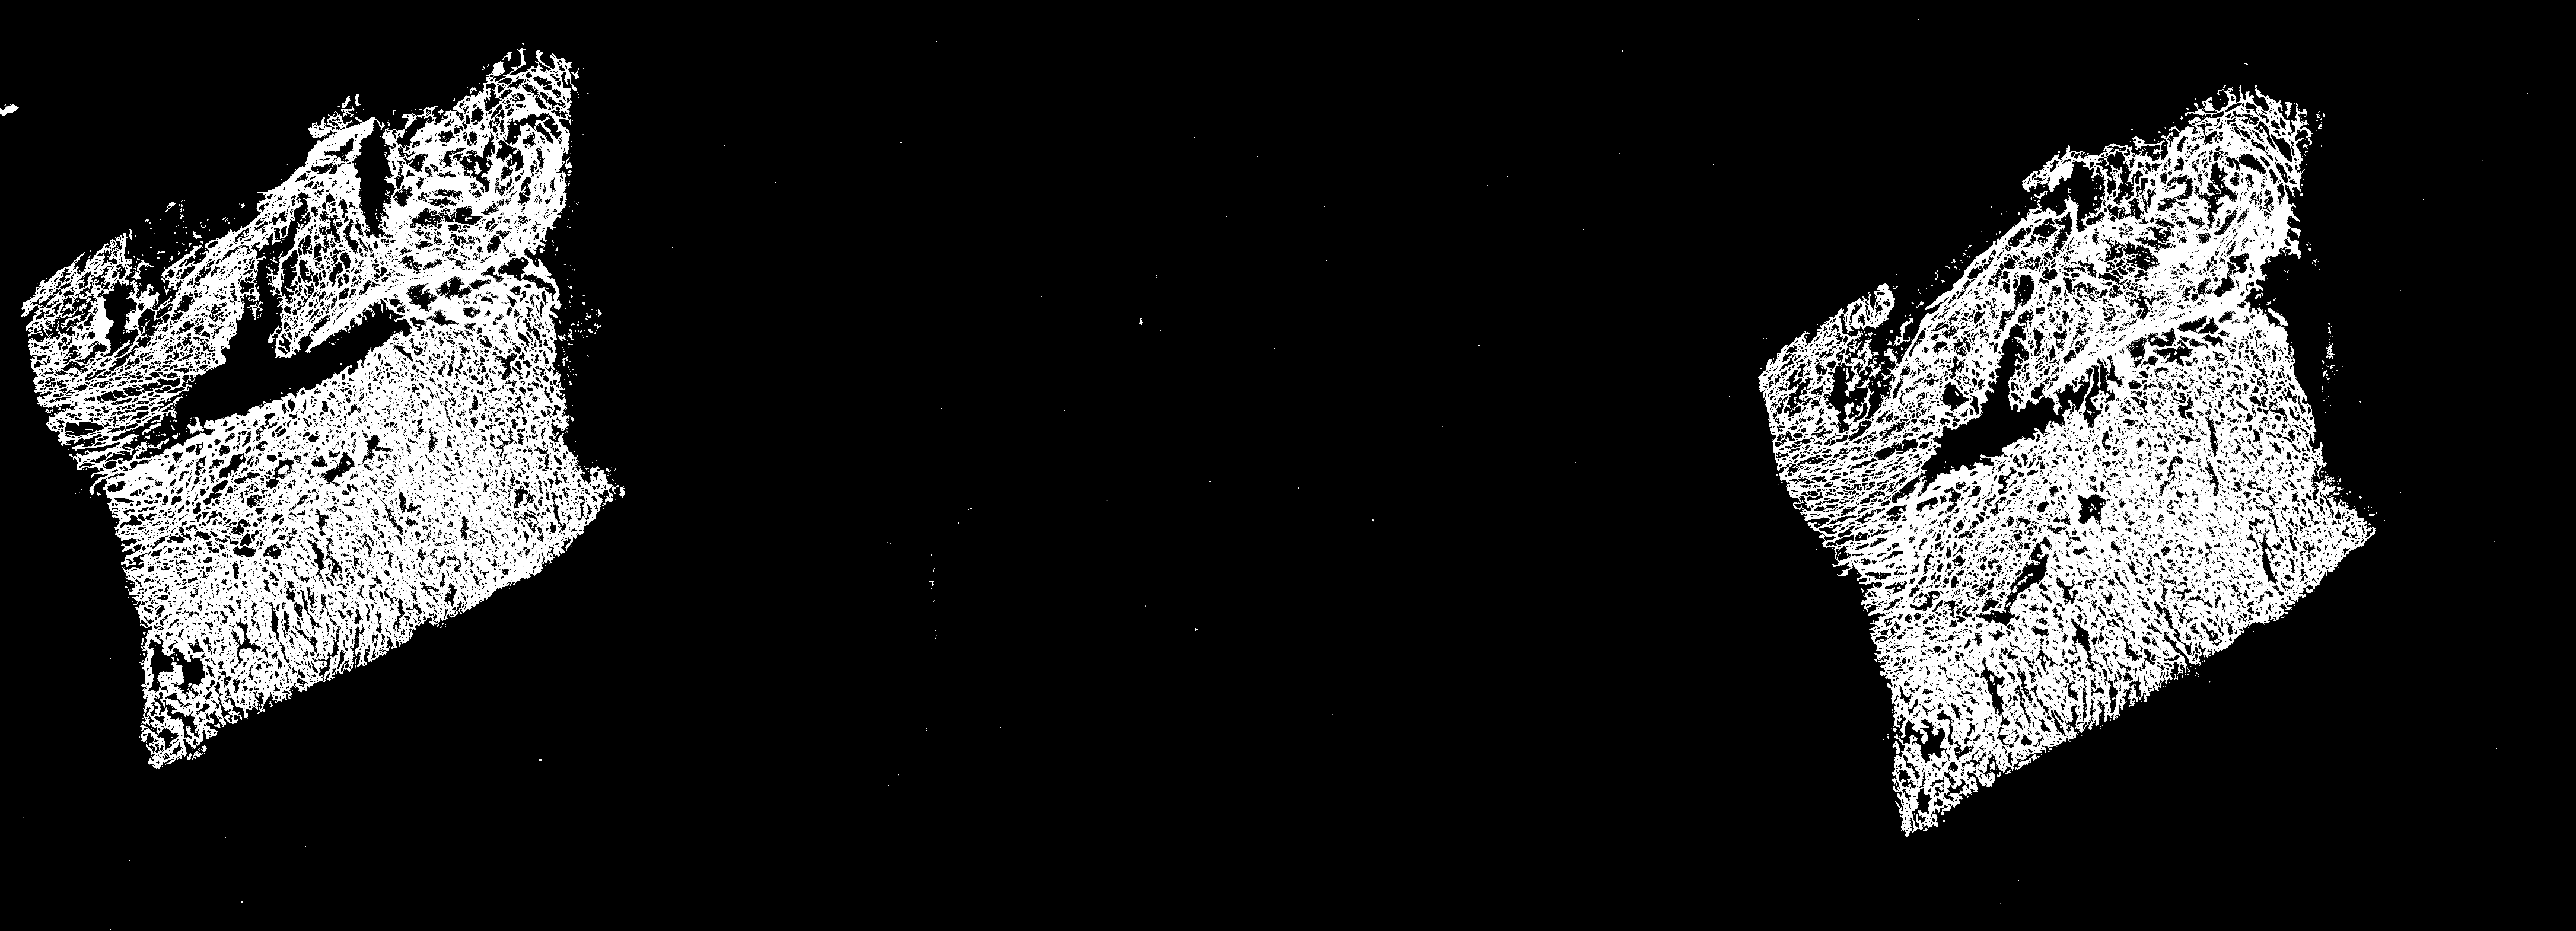
\includegraphics[width=0.48\linewidth]{figs/introduction/subs/challenges/evaluate_slides/TCGA-ET-A39N-01A-01-TSA.C38FCE19-9558-4035-9F0B-AD05B9BE321D___198_masked.png}
            \hspace{.2cm}
            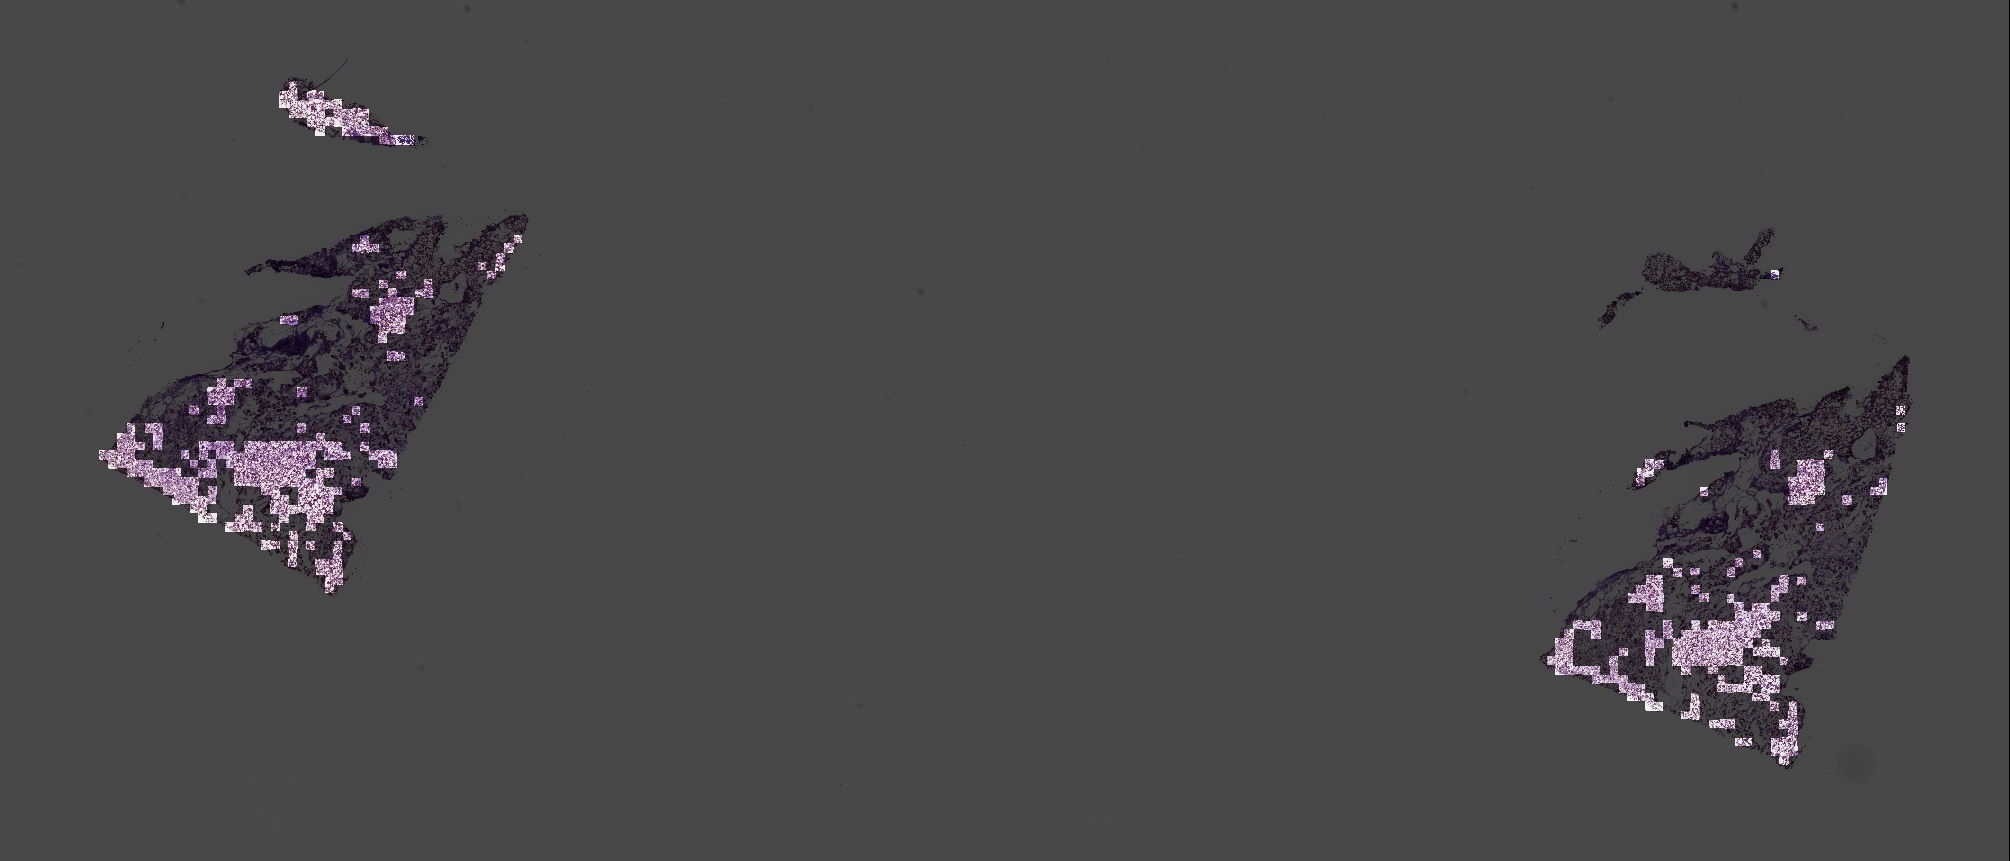
\includegraphics[width=0.48\linewidth]{figs/introduction/subs/challenges/evaluate_slides/TCGA-BJ-A3F0-01A-01-TSA.728CE583-95BE-462B-AFDF-FC0B228DF3DE__3_generated_mask.jpg}
            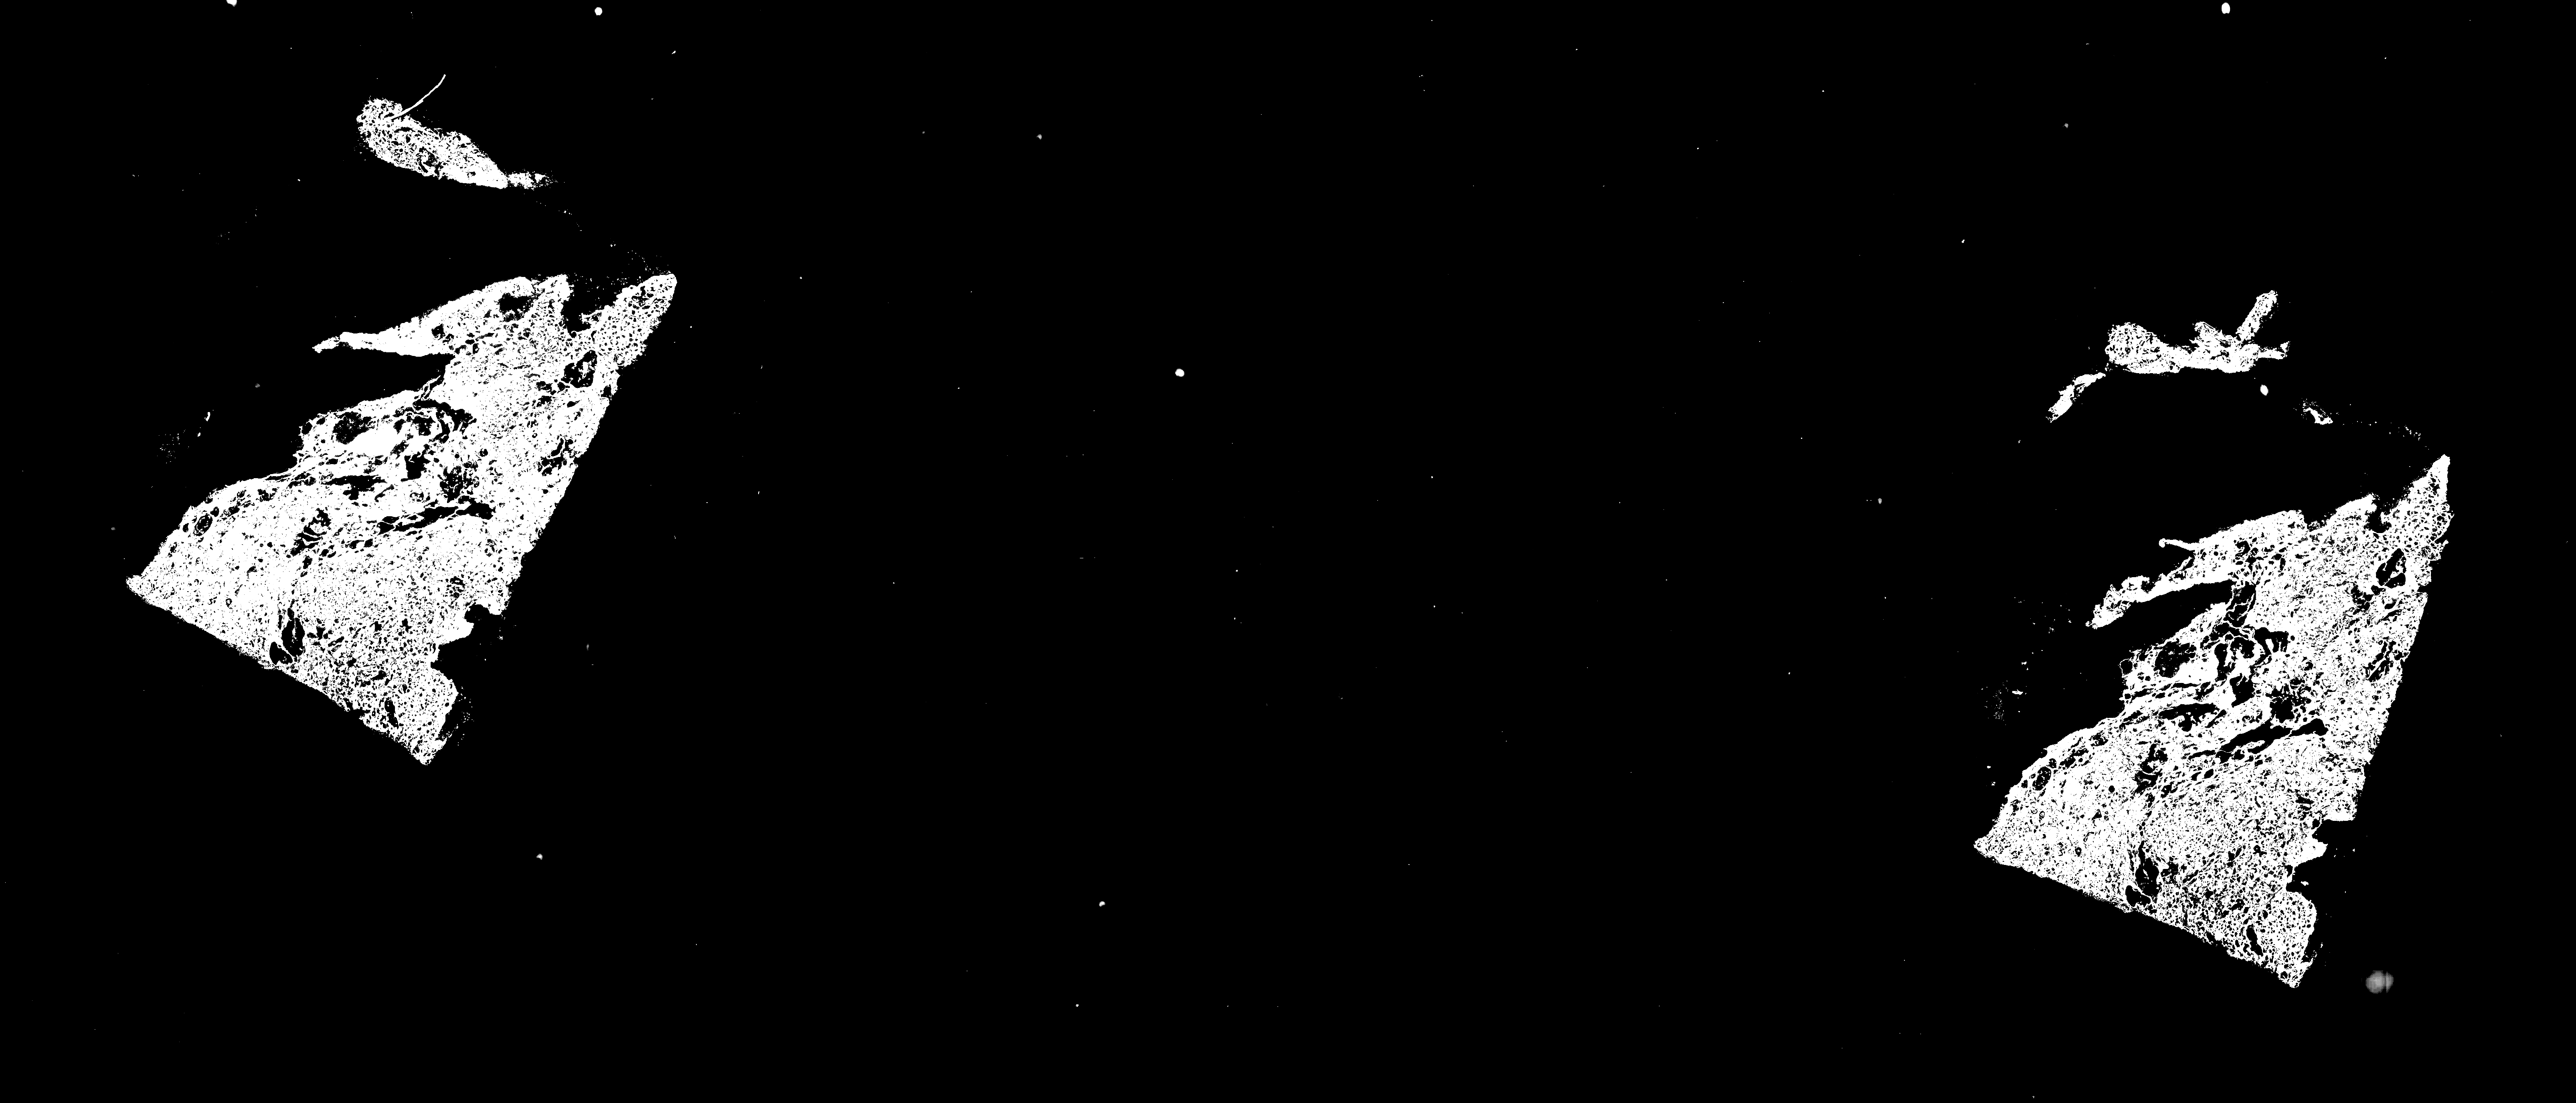
\includegraphics[width=0.48\linewidth]{figs/introduction/subs/challenges/evaluate_slides/TCGA-BJ-A3F0-01A-01-TSA.728CE583-95BE-462B-AFDF-FC0B228DF3DE__3_masked.png}
        \end{center}
        \caption{ناحیه‌های استخراج شده شش اسلاید $1$, $2$, $3$, $4$, $5$, $6$ در آستانه 298 و ماسک‌های مرتبط با آن‌ها}
        \label{شکل: شش اسلاید و ماسک‌های مرتبط}
    \end{figure}
\end{enumerate}
بعد از یافتن آستانه، می توان اسلاید‌ها را یکی پس از دیگری خواند و نواحی مورد نیاز برای آموزش مدل را استخراج کرد.
با توجه به توضیحات داده شده برای این روش استخراج، در ادامه به دو تا از مزیت‌های آن اشاره می کنیم:
\begin{itemize}
    \item از آنجایی که حجم داده ای که با آن‌ها کار داریم بسیار زیاد است و اسلاید‌های زیادی نیاز به پیش پردازش دارند سرعت و دقت عامل مهمی در عملکرد است.
    در این روش، بعد از تهیه ماسک‌ها برای شش اسلاید ذکر شده به صورت دستی و تعیین آستانه، دیگر نیاز به دخالت انسان نداریم، از این روی، این روش دقت و سرعت بالایی را داراست.
    \item همانطور که پیشتر نیز گفته شد، فایل‌های دیجیتال اسلاید‌ها، از طریق اسکن نمونه‌ها توسط دستگاه و در زیر میکروسکپ تهیه می شوند.
    در بعضی مواقع به دلیل شرایط فیزیکی نمونه، خطای دستگاه و یا حتی خطای انسانی ممکن است نمونه و یا قسمتی از آن به درستی اسکن نشود.
    این نواحی نیز علاوه بر نواحی پس زمینه اطلاعات مورد نیاز ما را ندارند و یا از دست داده اند و حالت بلوری به خود گرفته اند.
    با توجه به ماهیت روش استخراج ذکر شده، این مشکل در این فرآیند حل می شود.
    لاپلاسین یک تصویر حاوی اطلاعاتی نظیر گوشه‌ها و خطوط تصویر است از این روی، یکی از روش‌های اصلی تشخیص بلوری بودن تصویر است، زیرا در این تصاویر اطلاعاتی مانند خطوط محو می شوند.
    با توجه به اینکه مبنای اصلی روش استخراج ذکر شده نیز لاپلاسین تصویر است، در طی این فرآیند تصاویر بلوری مقدار واریانس لاپلاسین کمتری گرفته و خود به خود حذف می گردند.
\end{itemize}
